% Document
\documentclass[fontsize=8pt,paper=a4,paper=landscape,DIV=calc,]{scrartcl}
\usepackage[T1]{fontenc}
\usepackage{noto}
\usepackage[nswissgerman,english]{babel}
\renewcommand{\familydefault}{\sfdefault}

% Format
\usepackage[top=5mm,bottom=1mm,left=5mm,right=5mm,includehead]{geometry}
\setlength{\headheight}{\baselineskip}
\setlength{\headsep}{0mm}

\usepackage{multicol}
\setlength{\columnsep}{2mm}
\setlength{\columnseprule}{0.1pt}

% Color
\usepackage[svgnames]{xcolor}

% Math
\usepackage{amsmath}
\usepackage{amssymb}
\usepackage{amsfonts}
\newcommand*{\eq}{=}

%% Venn Diagrams
\usepackage{venndiagram}

%% Trees
%%% https://tex.stackexchange.com/a/425271
\usepackage{forest}
\forestset{
    ptree/.style={
        for tree={
            % grow'=0,
            % parent anchor=children,
            % child anchor=parent,
            grow'=east,
            parent anchor=east,
            child anchor=west,
            text width=7mm
        },
        before typesetting nodes={
            for tree={
                split option={content}{:}{content, my edge label},
            },
        },
    },
    my edge label/.style={
        if={
            > O_= {n'}{1}
        }{
            edge label={node [midway, below left, font=\tiny] {#1} }
        }{
            edge label={node [midway, above left, font=\tiny] {#1} }
        },
    }
}

% Standards
\newcommand{\rfc}[1]{\href{https://www.rfc-editor.org/rfc/rfc#1.html}{RFC#1}}
\newcommand{\ieee}[1]{\href{https://ieeexplore.ieee.org/search/searchresult.jsp?queryText=#1}{IEEExplore #1}}

% Code
\usepackage{listings}

\lstset{
   extendedchars=true,
   basicstyle=\footnotesize\ttfamily,
   tabsize=2,
   breaklines=true,
   showspaces=false,
   showtabs=false
   showstringspaces=false,
}

%% https://tex.stackexchange.com/a/536018
%% Allow for German characters in lstlistings.
\lstset{literate=
    {Ö}{{\"O}}1
    {Ä}{{\"A}}1
    {Ü}{{\"U}}1
    {ü}{{\"u}}1
    {ä}{{\"a}}1
    {ö}{{\"o}}1
}

%% Java Language definition
\lstdefinelanguage{java}{
  keywords=[1]{abstract, assert, boolean, byte, char, class, default, double,
  enum, extends, final, float, implements, import, instanceof, int, interface,
  long, native, null, package, private, protected, public, short, static,
  strictfp, super, synchronized, this, throw, throws, transient, void,
  volatile},
  keywordstyle=[1]\color{DarkBlue}\bfseries,
  keywords=[2]{if, else, while, do, try, case, catch, finally, new, break,
  continue, return, switch},
  keywordstyle=[2]\color{DarkRed}\bfseries,
  identifierstyle=\ttfamily,
  sensitive=false,
  comment=[l]{//},
  morecomment=[s]{/*}{*/},
  commentstyle=\color{DarkGray},
  stringstyle=\color{DarkGreen},
  morestring=[b]',
  morestring=[b]"
}

% Images
\usepackage{graphicx}
\graphicspath{{graphic/}}

% Links
\usepackage{hyperref}
\hypersetup{
    colorlinks=true,
    linkcolor=blue,
    filecolor=magenta,
    urlcolor=cyan,
}

% Smaller Lists
\usepackage{enumitem}
\setlist[itemize,enumerate]{leftmargin=3mm, labelindent=0mm, labelwidth=1mm, labelsep=1mm, nosep}
\setlist[description]{leftmargin=0mm, nosep}
\setlength{\parindent}{0cm}

% Smaller Titles
\usepackage[explicit]{titlesec}

%% Color Boxes
\newcommand{\sectioncolor}[1]{\colorbox{black!60}{\parbox{0.97\linewidth}{\color{white}#1}}}
\newcommand{\subsectioncolor}[1]{\colorbox{black!50}{\parbox{0.97\linewidth}{\color{white}#1}}}
\newcommand{\subsubsectioncolor}[1]{\colorbox{black!40}{\parbox{0.97\linewidth}{\color{white}#1}}}
\newcommand{\paragraphcolor}[1]{\colorbox{black!30}{\parbox{0.97\linewidth}{\color{white}#1}}}
\newcommand{\subparagraphcolor}[1]{\colorbox{black!20}{\parbox{0.97\linewidth}{\color{white}#1}}}

%% Title Format
\titleformat{\section}{\vspace{0.5mm}\bfseries}{}{0mm}{\sectioncolor{\thesection~#1}}[{\vspace{0.5mm}}]
\titleformat{\subsection}{\vspace{0.5mm}\bfseries}{}{0mm}{\subsectioncolor{\thesubsection~#1}}[{\vspace{0.5mm}}]
\titleformat{\subsubsection}{\vspace{0.5mm}\bfseries}{}{0mm}{\subsubsectioncolor{\thesubsubsection~#1}}[{\vspace{0.5mm}}]
\titleformat{\paragraph}{\vspace{0.5mm}\bfseries}{}{0mm}{\paragraphcolor{\theparagraph~#1}}[{\vspace{0.5mm}}]
\titleformat{\subparagraph}{\vspace{0.5mm}\bfseries}{}{0mm}{\subparagraphcolor{\thesubparagraph~#1}}[{\vspace{0.5mm}}]

%% Title Spacing
\titlespacing{\section}{0mm}{0mm}{0mm}
\titlespacing{\subsection}{0mm}{0mm}{0mm}
\titlespacing{\subsubsection}{0mm}{0mm}{0mm}
\titlespacing{\paragraph}{0mm}{0mm}{0mm}
\titlespacing{\subparagraph}{0mm}{0mm}{0mm}

%define header and footer
\usepackage{fancyhdr}
\pagestyle{fancy}

\fancyhead[RO]{\AUTHOR\hspace{4pt}|\hspace{4pt}\INSTITUTE}
\fancyhead[LO]{\TITLE}
\usepackage[style=iso]{datetime2}
\fancyfoot[RO]{\today}
\renewcommand\headrulewidth{0pt}
\renewcommand\footrulewidth{0pt}
\headsep = -2pt
\footskip = 0pt

% no vertical distribution
%% explanation: we copy the macro columnbreak to stdcolumnbreak
%% we now redefine columnbreak to always fill up null space and then execute the standard columnbreak.
\let\stdcolumnbreak\columnbreak
\renewcommand\columnbreak{\vfill\null\stdcolumnbreak}


\newcommand{\TITLE}{Betriebssysteme 1}
\newcommand{\AUTHOR}{Mona Panchaud}
\newcommand{\INSTITUTE}{Ostschweizer Fachhochschule}
\begin{document}
\begin{multicols*}{4}

\section{Prozessor}
P. kann nur über Speicherbus mit Umwelt interagieren!
\textbf{schreiben}:
\begin{enumerate}
    \item P. legt Adresse auf Adressbus \& Daten auf Datenbus
    \item P. aktiviert Speicherbus zum Schreiben
\end{enumerate}
\textbf{lesen}:
\begin{enumerate}
    \item P. legt Adresse auf Adressbus
    \item P. aktiviert Speicherbus zum Lesen
    \item Speicher legt Daten auf Datenbus
\end{enumerate}
OpCode: 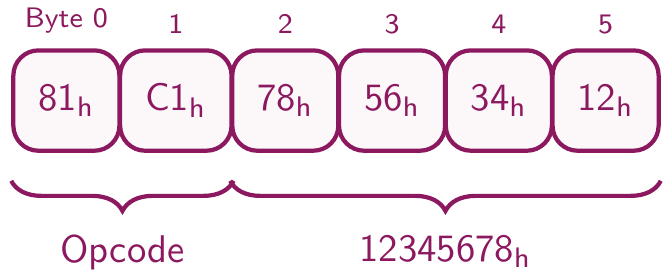
\includegraphics[width=0.1\textwidth]{opcode.png}

\section{Numbers in Assembly}
\begin{description}
    \item[db] Byte, 8 Bit
    \item[dw] Word, 2 Byte, 16 Bit
    \item[dd] Doubleword, 4 Byte, 32 Bit
    \item[dq] Quadword, 8 Byte, 64 Bit
    \item [Double Quadword] 16 Byte, 128 Bit
\end{description}

\section{Byte Order}
Stellen innerhalb Bytes werden nicht vertauscht!
\begin{description}
    \item[Big-Endian] CA | FE -> MSB ist erstes Bit
    \item[Little-Endian] FE | CA -> LSB ist erstes Bit
\end{description}

\section{Labels}
\begin{lstlisting}[language={[x86masm]Assembler}]
text_length: dq after_my_text - my_text
my_text: db 'BSys 1'
after_my_text:
\end{lstlisting}

\section{Register}
\begin{tabular}{llllll}
    63..0 & 31..0 & 15..0 & 15..8 & 7..0\\
    \hline
    RAX & EAX & AX & AH & AL\\
\end{tabular}

\textbf{Weitere:} RCX, RDX, RBX, RSI, RDI, RSP, RBP, R8-R15

% TODO add syscall somewhere?

\section{Memory}
% TODO do I have enough space to add Displacement Adressierung, Scaled-Index-Adressierung & Base Adressierung?
\begin{lstlisting}[language={[x86masm]Assembler}]
mov rax, [0x8000] ; move 8000h into rax
mov rbx, [rax] ; address is in the register rax
mov [0x8000], rax ; move val at rax into 0x8000
; move rbx into rax, no memory access:
mov rax, rbx
; error can't move memory to memory:
mov [0x8000], [0x7000]
\end{lstlisting}
Operanden müssen gleich gross sein.

% TODO: More Assembly constructs
% (e.g. arithmetic operations)
% see saved pages

% TODO take a look later if "subsection" is correct
\subsection{Flags}
CF \& OF werden immer beide von CPU bestimmt.

Carry Flag (CF) == Überlauf bei \textbf{unsigned} Arithmetik

0001 + 1111 = 0000, CF = 1 --> 1 + 15 = 0, CF = 1

Overflow Flag (OF) == Überlauf bei \textbf{signed} Arithmetik

0111 + 0001 = 1000 -> 7 + 1 = -8 (negative prefix)

Zero Flag (ZF) == set when result is 0

Sign Flag == is the highest bit of the result

Parity Flag (PF) == set if lowest byte has even number of bits

\section{Stack (\& Framepointer)}
"Oberstes" Element an kleinster Adresse

-> wächst nach unten

Prozessor überprüft \textbf{keine} obere/untere Grenze!

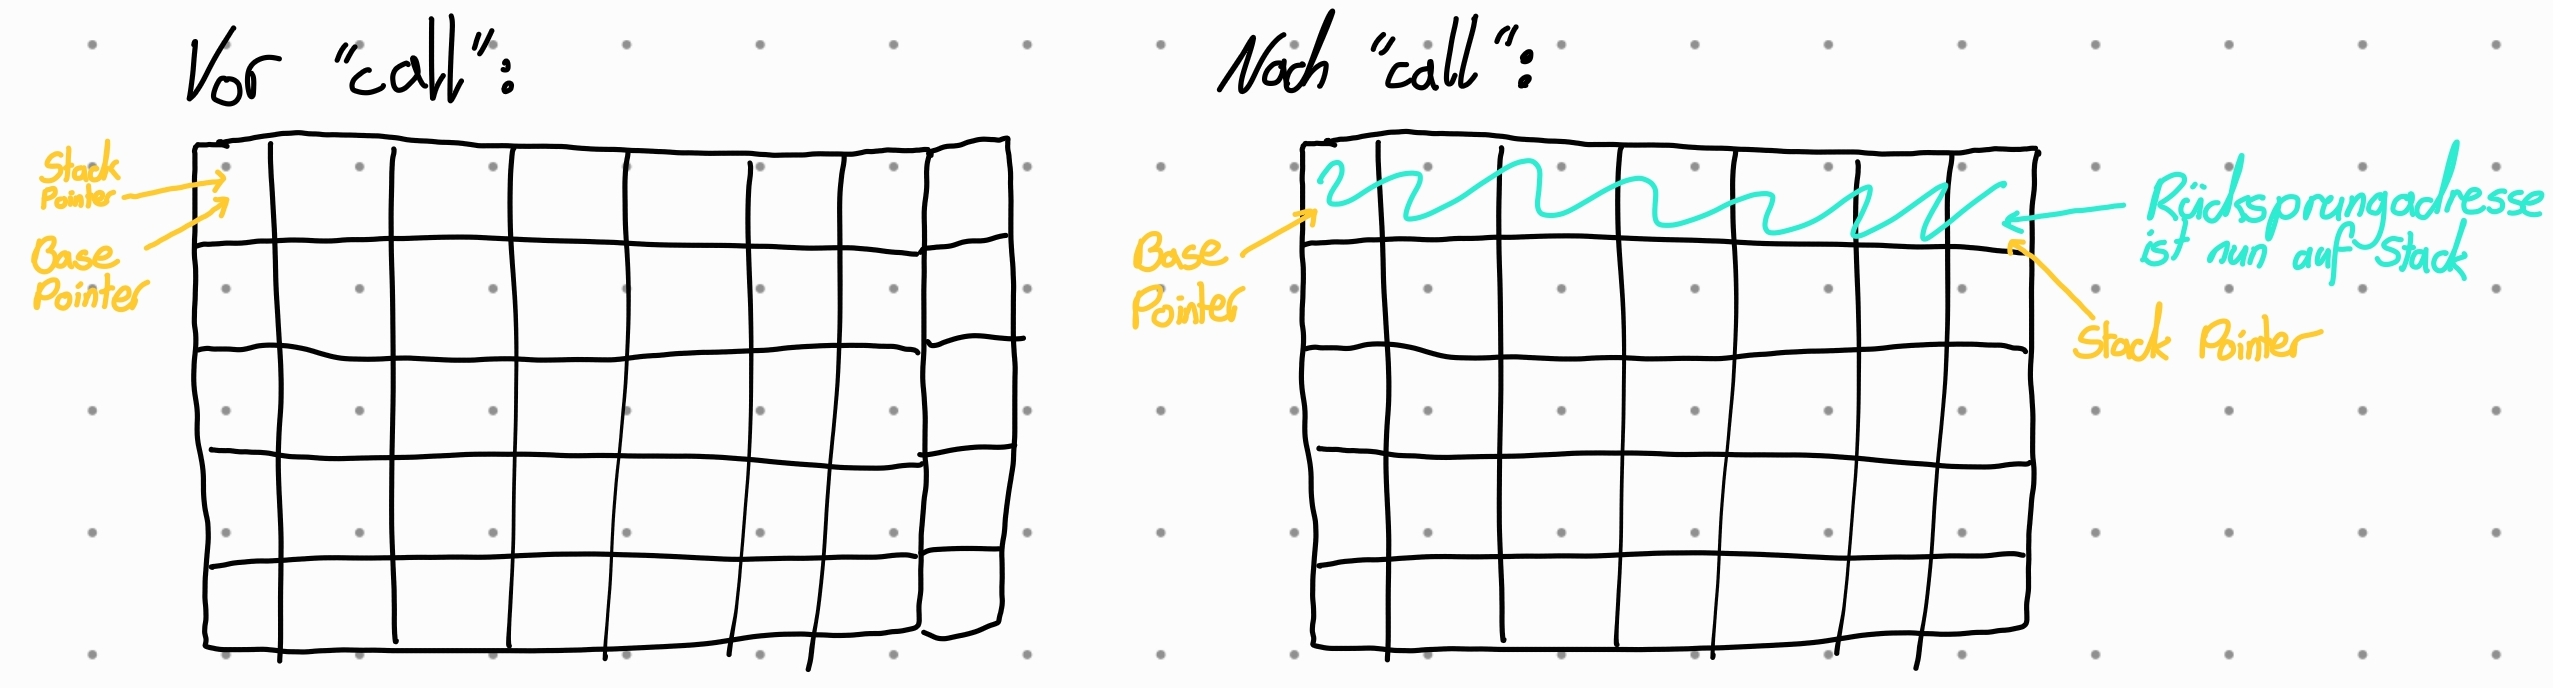
\includegraphics[width=0.25\textwidth]{rbp_rsp_base_sit.jpg}
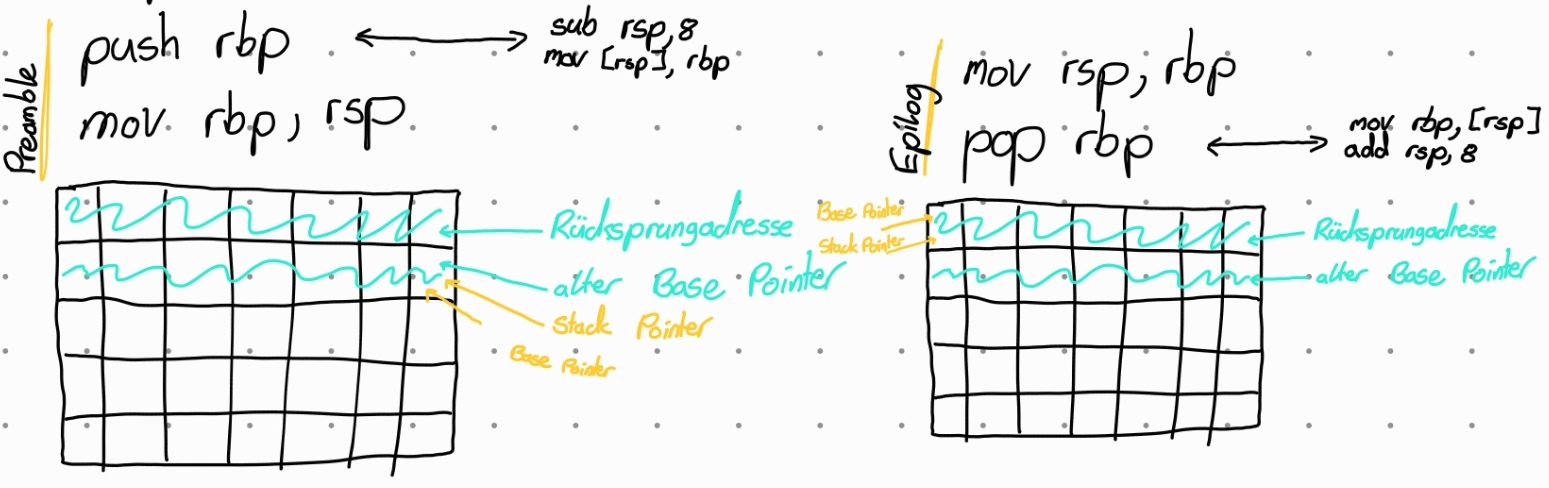
\includegraphics[width=0.24\textwidth]{rbp_rsp_preamble_epilogue.jpg}

Argumente sind vor der Rücksprungadresse auf Stack gelandet. Access via: [rbp + 0x10]

\section{Calling Conventions}
Welche Register / Stack für Argumente.

Von Betriebssystem / Compiler bestimmt => unterschiedlich

\section{C}
\subsection{C-Toolchain}
\begin{enumerate}
    \item \textbf{C Präprozessor} -> Bereinigte C-Quelle
    \item \textbf{C Compiler} -> Assembler Datei
    \item \textbf{Assembler} -> Objekt Datei
    \item \textbf{Linker} -> Executable
\end{enumerate}
\subsubsection{Präprozessor}
\begin{enumerate}
    \item Kommentare entfernen \& \ Zeilen zusammensetzen
    \item In Tokens aufteilen (Whitespace, bei a+b nicht nötig, String wird nicht aufgeteilt).

    Bildet grösstmögliches Token
    \item Präprozessor Direktiven ausführen (include, if, ...)

    \& Makros expandieren
\end{enumerate}
\begin{lstlisting}[language=c]
#define XYZ 123
// XYZ wird im Folgenden mit 123 ersetzt
\end{lstlisting}

\subsubsection{Compiler}
Eine C-Datei -> Eine Assemblerdatei

Bezeichner dürfen beliebig oft \underline{deklariert} (int y;) werden. Nur 1x \underline{definiert} (int y = 5;).

\textbf{static}: Variable, die nicht exportiert werden soll

\begin{lstlisting}[language=c]
extern int x; static int x = 5; // Error:
// static Deklaration folgt auf non-static
\end{lstlisting}

Für globale Var wird Speicher fix reserviert. Grösse hängt von Typ ab. globale Var werden exportiert.

\subsubsection{Linker}
Mehrere Assemblerdateien -> Ein Executable

\subsection{Typen, sizeof(t)}
Typinfos nur auf C Sprachlevel

Size infos are dependent on architecture

\subsection{Vorzeichen}
Bei signed MSB: 0=positiv, 1=negativ

Umwandlung von negativer Binärzahl:

Zweierkomplement bilden -> flip + 1

-> 1010 -> 0101 -> 0110

\subsection{Pointers}

\begin{lstlisting}[language=c]
int a = 42;
int *b = &a; // b pointer to a
a = *b + 1; // a = dereference b and add 1
\end{lstlisting}
Incrementing a pointer will skip \textbf{sizeof(t)} Bytes!

\subsection{Numbers in C}
\begin{itemize}
    \item Decimal: 0..9 with \textbf{NO 0 at the start}
    \item Octal: 0..7 with a \textbf{leading 0}
    \item Hex: 0..F with \textbf{leading 0x}
    \item Suffix: the suffic specifies a type:

    l: long, ll: long long, u: unsigned, ul: unsigned long
\end{itemize}

\subsection{Bitwise Operators}
Werden Bit per Bit angewendet:

not: \~{}q | and: q \& p | or: q | p

left shift: q << p ($* 2^m$) | right shift: q >> p ("$/ 2^m$")
\subsection{Logische Operatoren}
not: !q | and: q \&\& p | or: q || p

\subsection{Arithmetische Operationen}
z = x + y -> falls Überlauf: verpufft (kein Carry)

\subsection{Funktionen}
Parameter werden immer kopiert. (call by value)\vspace{2pt}

Bei Pointer als Parameter: Pointer wird kopiert, nicht der Wert dahinter -> Simulation von call by reference.\vspace{2pt}

Rückgabewert kann jeder Typ ausser Array Typen sein. Rückgabewert wird immer kopiert.

\begin{lstlisting}[language=c]
void f ();
void g (void);
f(); // OK
g(); // OK
f(1, 2, 3); // OK. LOL.
g(1, 2, 3); // Fehler -> parameter type is void
\end{lstlisting}

\subsection{printf Identifiers}
\begin{itemize}
    \item \textcolor{teal}{sizeof(Integer) as signed decimal = \%d}
    \item \textcolor{teal}{sizeof(Integer) as unsigned decimal = \%u}
    \item \textcolor{teal}{sizeof(Integer) as hexadecimal = \%x or \%U}
    \item \textcolor{teal}{sizeof(long) as signed decimal = \%li}
    \item \textcolor{teal}{sizeof(long long) as signed decimal = \%lli}
    \item \textcolor{teal}{sizeof(void *) as pointer = \%p}
    \item \textcolor{teal}{sizeof(char *) as pointer (null terminated) = \%s}
    \item \textcolor{teal}{sizeof(double) as floating point = \%f}
\end{itemize}

\end{multicols*}
\end{document}
